% Shared float (common/make_floats.py). Figure: figures/generative_sampling.pdf
\begin{figure}[htbp]
\centering
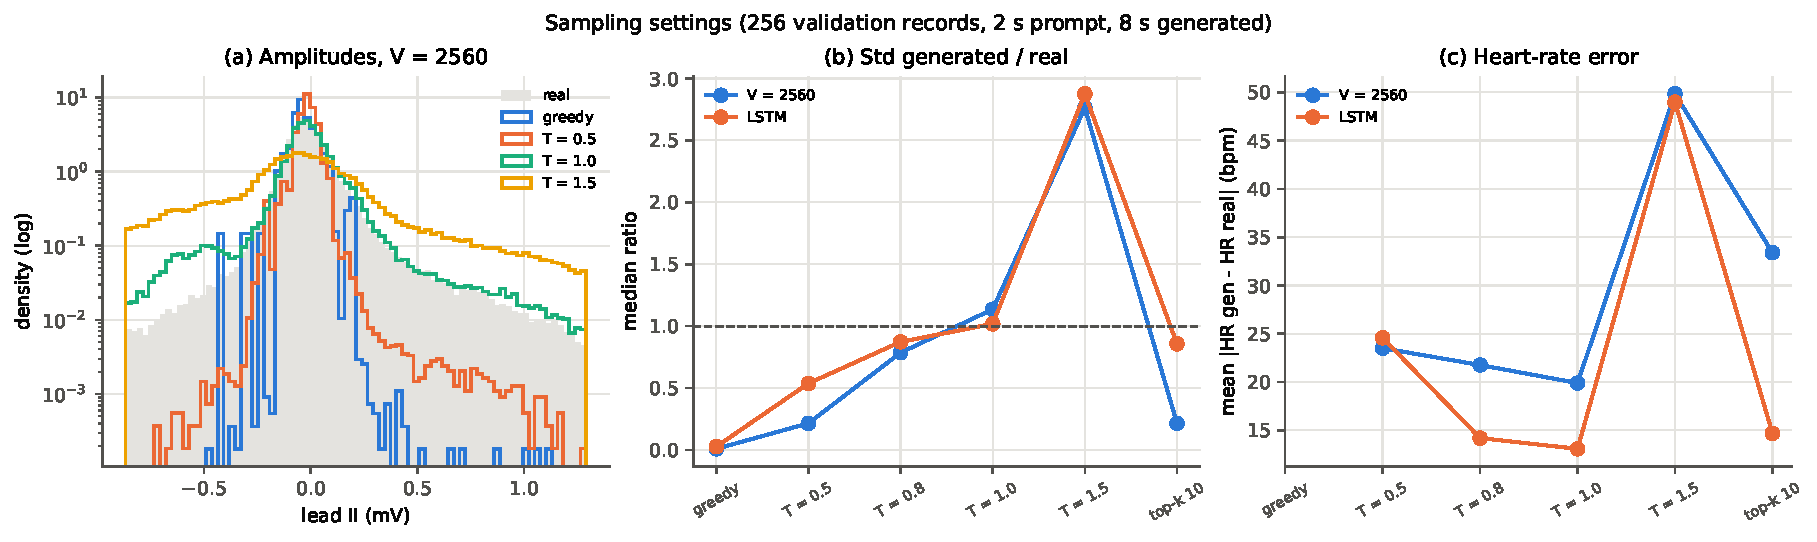
\includegraphics[width=\textwidth,height=0.42\textheight,keepaspectratio]{figures/generative_sampling.pdf}
\caption[Generators: sampling settings]{Sampling settings (256 validation records, 2\,s prompt, 8\,s generated). (a) Amplitude distributions of the generated signals against the real ones ($V = 2560$). (b) Median ratio of generated to real standard deviation. (c) Mean absolute heart-rate error.}
\label{fig:generative_sampling}
\end{figure}
